% Options for packages loaded elsewhere
% Options for packages loaded elsewhere
\PassOptionsToPackage{unicode}{hyperref}
\PassOptionsToPackage{hyphens}{url}
\PassOptionsToPackage{dvipsnames,svgnames,x11names}{xcolor}
%
\documentclass[
  french,
  11pt,
  a4paper,
]{article}
\usepackage{xcolor}
\usepackage[top=1.5cm, bottom=1.5cm, left=2.5cm, right=2.5cm]{geometry}
\usepackage{amsmath,amssymb}
\setcounter{secnumdepth}{-\maxdimen} % remove section numbering
\usepackage{iftex}
\ifPDFTeX
  \usepackage[T1]{fontenc}
  \usepackage[utf8]{inputenc}
  \usepackage{textcomp} % provide euro and other symbols
\else % if luatex or xetex
  \usepackage{unicode-math} % this also loads fontspec
  \defaultfontfeatures{Scale=MatchLowercase}
  \defaultfontfeatures[\rmfamily]{Ligatures=TeX,Scale=1}
\fi
\usepackage{lmodern}
\ifPDFTeX\else
  % xetex/luatex font selection
\fi
% Use upquote if available, for straight quotes in verbatim environments
\IfFileExists{upquote.sty}{\usepackage{upquote}}{}
\IfFileExists{microtype.sty}{% use microtype if available
  \usepackage[]{microtype}
  \UseMicrotypeSet[protrusion]{basicmath} % disable protrusion for tt fonts
}{}
\makeatletter
\@ifundefined{KOMAClassName}{% if non-KOMA class
  \IfFileExists{parskip.sty}{%
    \usepackage{parskip}
  }{% else
    \setlength{\parindent}{0pt}
    \setlength{\parskip}{6pt plus 2pt minus 1pt}}
}{% if KOMA class
  \KOMAoptions{parskip=half}}
\makeatother
% Make \paragraph and \subparagraph free-standing
\makeatletter
\ifx\paragraph\undefined\else
  \let\oldparagraph\paragraph
  \renewcommand{\paragraph}{
    \@ifstar
      \xxxParagraphStar
      \xxxParagraphNoStar
  }
  \newcommand{\xxxParagraphStar}[1]{\oldparagraph*{#1}\mbox{}}
  \newcommand{\xxxParagraphNoStar}[1]{\oldparagraph{#1}\mbox{}}
\fi
\ifx\subparagraph\undefined\else
  \let\oldsubparagraph\subparagraph
  \renewcommand{\subparagraph}{
    \@ifstar
      \xxxSubParagraphStar
      \xxxSubParagraphNoStar
  }
  \newcommand{\xxxSubParagraphStar}[1]{\oldsubparagraph*{#1}\mbox{}}
  \newcommand{\xxxSubParagraphNoStar}[1]{\oldsubparagraph{#1}\mbox{}}
\fi
\makeatother


\usepackage{longtable,booktabs,array}
\newcounter{none} % for unnumbered tables
\usepackage{calc} % for calculating minipage widths
% Correct order of tables after \paragraph or \subparagraph
\usepackage{etoolbox}
\makeatletter
\patchcmd\longtable{\par}{\if@noskipsec\mbox{}\fi\par}{}{}
\makeatother
% Allow footnotes in longtable head/foot
\IfFileExists{footnotehyper.sty}{\usepackage{footnotehyper}}{\usepackage{footnote}}
\makesavenoteenv{longtable}
\usepackage{graphicx}
\makeatletter
\newsavebox\pandoc@box
\newcommand*\pandocbounded[1]{% scales image to fit in text height/width
  \sbox\pandoc@box{#1}%
  \Gscale@div\@tempa{\textheight}{\dimexpr\ht\pandoc@box+\dp\pandoc@box\relax}%
  \Gscale@div\@tempb{\linewidth}{\wd\pandoc@box}%
  \ifdim\@tempb\p@<\@tempa\p@\let\@tempa\@tempb\fi% select the smaller of both
  \ifdim\@tempa\p@<\p@\scalebox{\@tempa}{\usebox\pandoc@box}%
  \else\usebox{\pandoc@box}%
  \fi%
}
% Set default figure placement to htbp
\def\fps@figure{htbp}
\makeatother



\ifLuaTeX
\usepackage[bidi=basic,shorthands=off]{babel}
\else
\usepackage[bidi=default,shorthands=off]{babel}
\fi
\ifLuaTeX
  \usepackage{selnolig} % disable illegal ligatures
\fi


\setlength{\emergencystretch}{3em} % prevent overfull lines

\providecommand{\tightlist}{%
  \setlength{\itemsep}{0pt}\setlength{\parskip}{0pt}}



 


\usepackage{setspace}
\onehalfspacing
\usepackage{indentfirst}
\setlength{\parindent}{2em}
\setlength{\parskip}{1em}
\makeatletter
\@ifpackageloaded{caption}{}{\usepackage{caption}}
\AtBeginDocument{%
\ifdefined\contentsname
  \renewcommand*\contentsname{Table des matières}
\else
  \newcommand\contentsname{Table des matières}
\fi
\ifdefined\listfigurename
  \renewcommand*\listfigurename{Liste des Figures}
\else
  \newcommand\listfigurename{Liste des Figures}
\fi
\ifdefined\listtablename
  \renewcommand*\listtablename{Liste des Tables}
\else
  \newcommand\listtablename{Liste des Tables}
\fi
\ifdefined\figurename
  \renewcommand*\figurename{Figure}
\else
  \newcommand\figurename{Figure}
\fi
\ifdefined\tablename
  \renewcommand*\tablename{Table}
\else
  \newcommand\tablename{Table}
\fi
}
\@ifpackageloaded{float}{}{\usepackage{float}}
\floatstyle{ruled}
\@ifundefined{c@chapter}{\newfloat{codelisting}{h}{lop}}{\newfloat{codelisting}{h}{lop}[chapter]}
\floatname{codelisting}{Listing}
\newcommand*\listoflistings{\listof{codelisting}{Liste des Listings}}
\makeatother
\makeatletter
\makeatother
\makeatletter
\@ifpackageloaded{caption}{}{\usepackage{caption}}
\@ifpackageloaded{subcaption}{}{\usepackage{subcaption}}
\makeatother
\usepackage{bookmark}
\IfFileExists{xurl.sty}{\usepackage{xurl}}{} % add URL line breaks if available
\urlstyle{same}
\hypersetup{
  pdflang={fr},
  colorlinks=true,
  linkcolor={blue},
  filecolor={Maroon},
  citecolor={Blue},
  urlcolor={Blue},
  pdfcreator={LaTeX via pandoc}}


\author{}
\date{}
\begin{document}


\begin{titlepage}
\centering

\includegraphics{Ensai-logo.png}\\
\vspace{1cm}
{\LARGE\textsc{Ensai Cinema Club}}\\

\vspace{2cm}

\rule{\textwidth}{0.5mm}\\
\vspace {0.3cm}
{\huge\bfseries Analysis File}\\
\vspace {0.5cm}

\rule{\textwidth}{0.5mm}\\



\vspace{3cm}

\begin{flushleft}
\emph{Étudiants:}\\
N. Bougis,\\
S. Mironescu \\
Z. Goulamaly \\
S. Harris
\end{flushleft}


\begin{flushright}
\emph{Tuteur:}\\
C. Valot\\
\end{flushright}

\vfill 
\begin{center}
École Nationale de la Statistique et de l’Analyse de l’Information\\
2025--2026
\end{center}
\end{titlepage}

\newpage

\renewcommand{\contentsname}{Summary}
\tableofcontents

\newpage

\section{Introduction}\label{introduction}

\emph{{[}Project context, initial problem statement, overall objectives,
brief presentation of the intended final product, announcement of the
outline.{]}}

\begin{center}\rule{0.5\linewidth}{0.5pt}\end{center}

\section{Part 1 -- Functional
Analysis}\label{part-1-functional-analysis}

\subsection{Rephrasing the
requirements}\label{rephrasing-the-requirements}

\subsection{Selected features}\label{selected-features}

\subsubsection{Priority features}\label{priority-features}

\subsubsection{Features included if time
allows}\label{features-included-if-time-allows}

\subsubsection{Features excluded}\label{features-excluded}

\subsection{Summary: Use case diagram}\label{summary-use-case-diagram}

\begin{figure}

\centering{

\pandocbounded{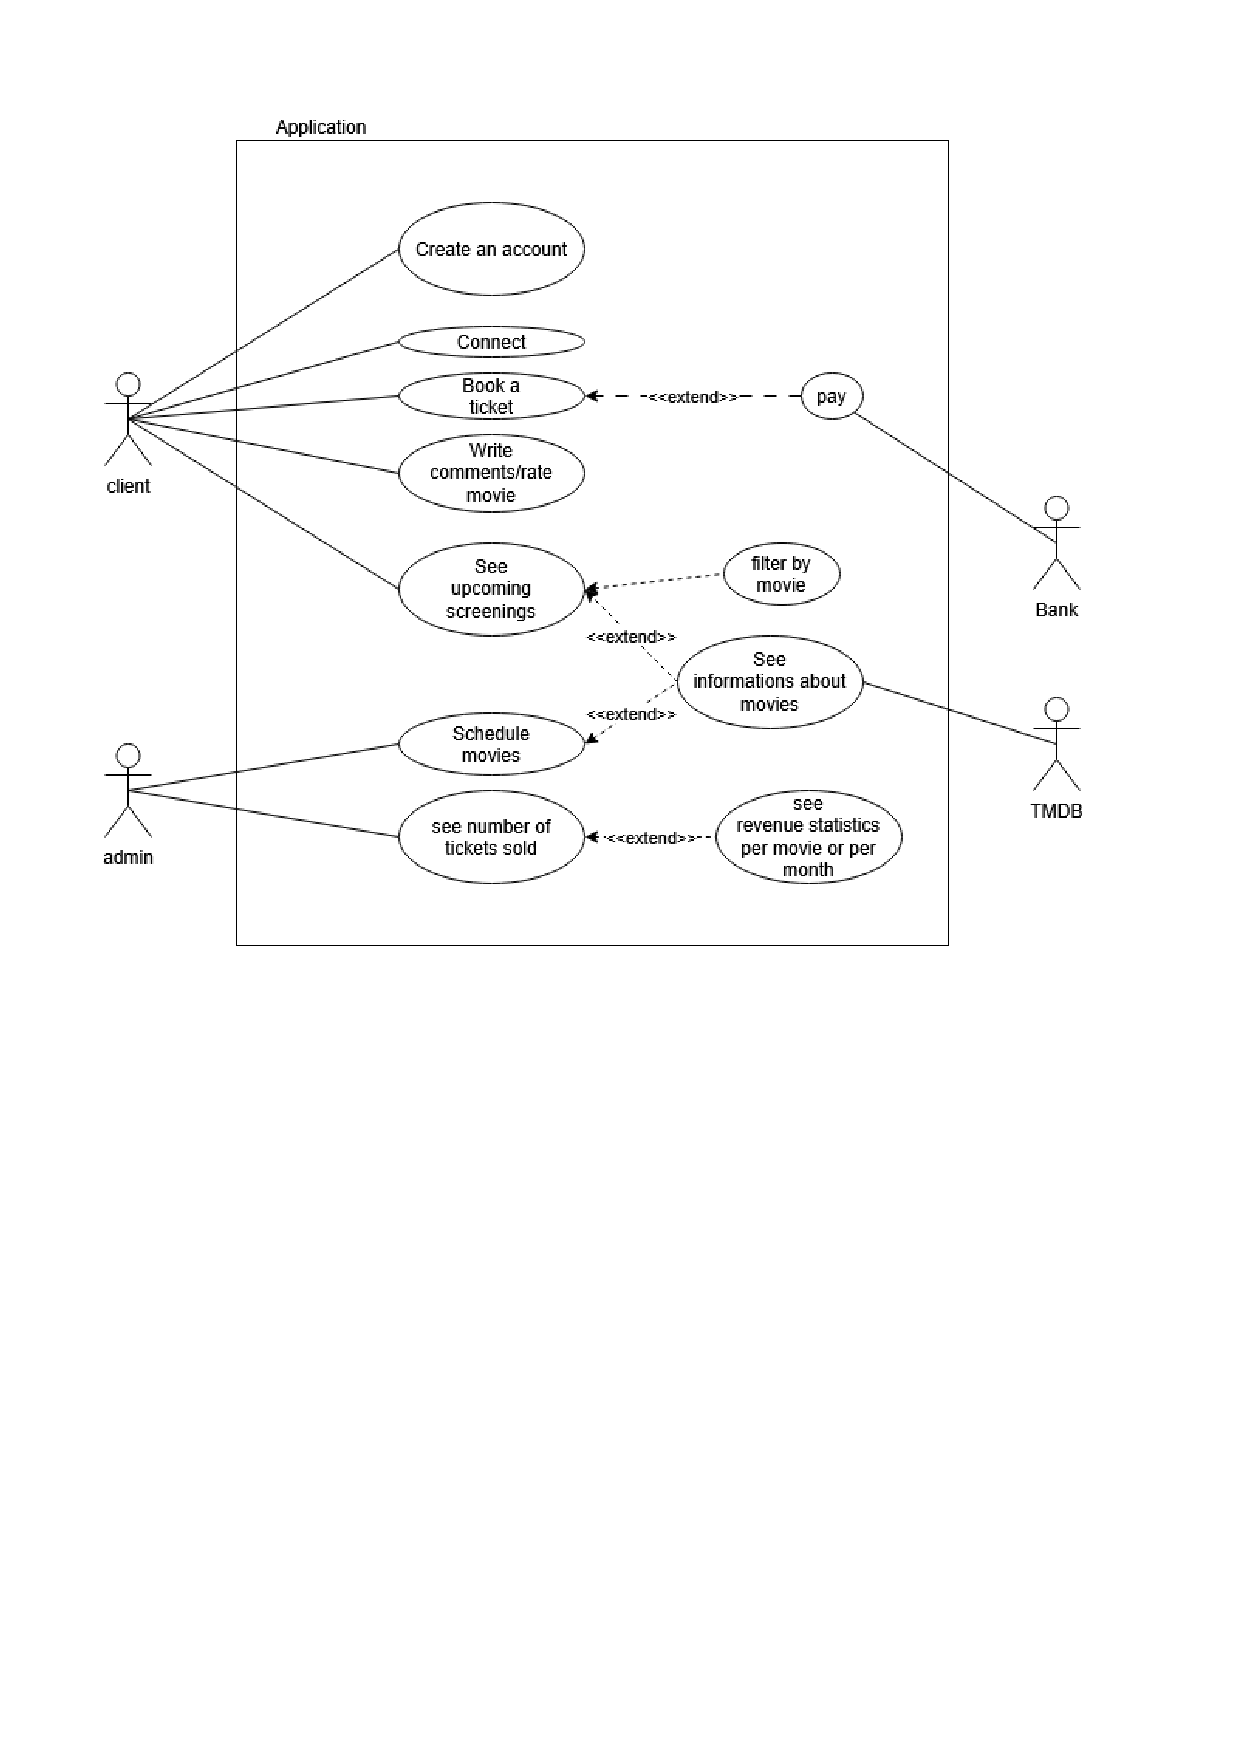
\includegraphics[keepaspectratio]{use-case-diagram.pdf}}

}

\caption{\label{fig-usecase}Use case diagram}

\end{figure}%

\section{Part 2 -- Technical-Functional
Layout}\label{part-2-technical-functional-layout}

\subsection{Benchmark of the Movie Information
API}\label{benchmark-of-the-movie-information-api}

\subsection{Overall structure and integration with third-party
services}\label{overall-structure-and-integration-with-third-party-services}

\subsection{Justification of technical
choices}\label{justification-of-technical-choices}

\section{Part 3 -- Technical Design}\label{part-3-technical-design}

\subsection{Architecture diagram}\label{architecture-diagram}

\emph{{[}Detailed technical view: application layers, frameworks,
hosting, communication between components.{]}}

\begin{figure}

\centering{

\pandocbounded{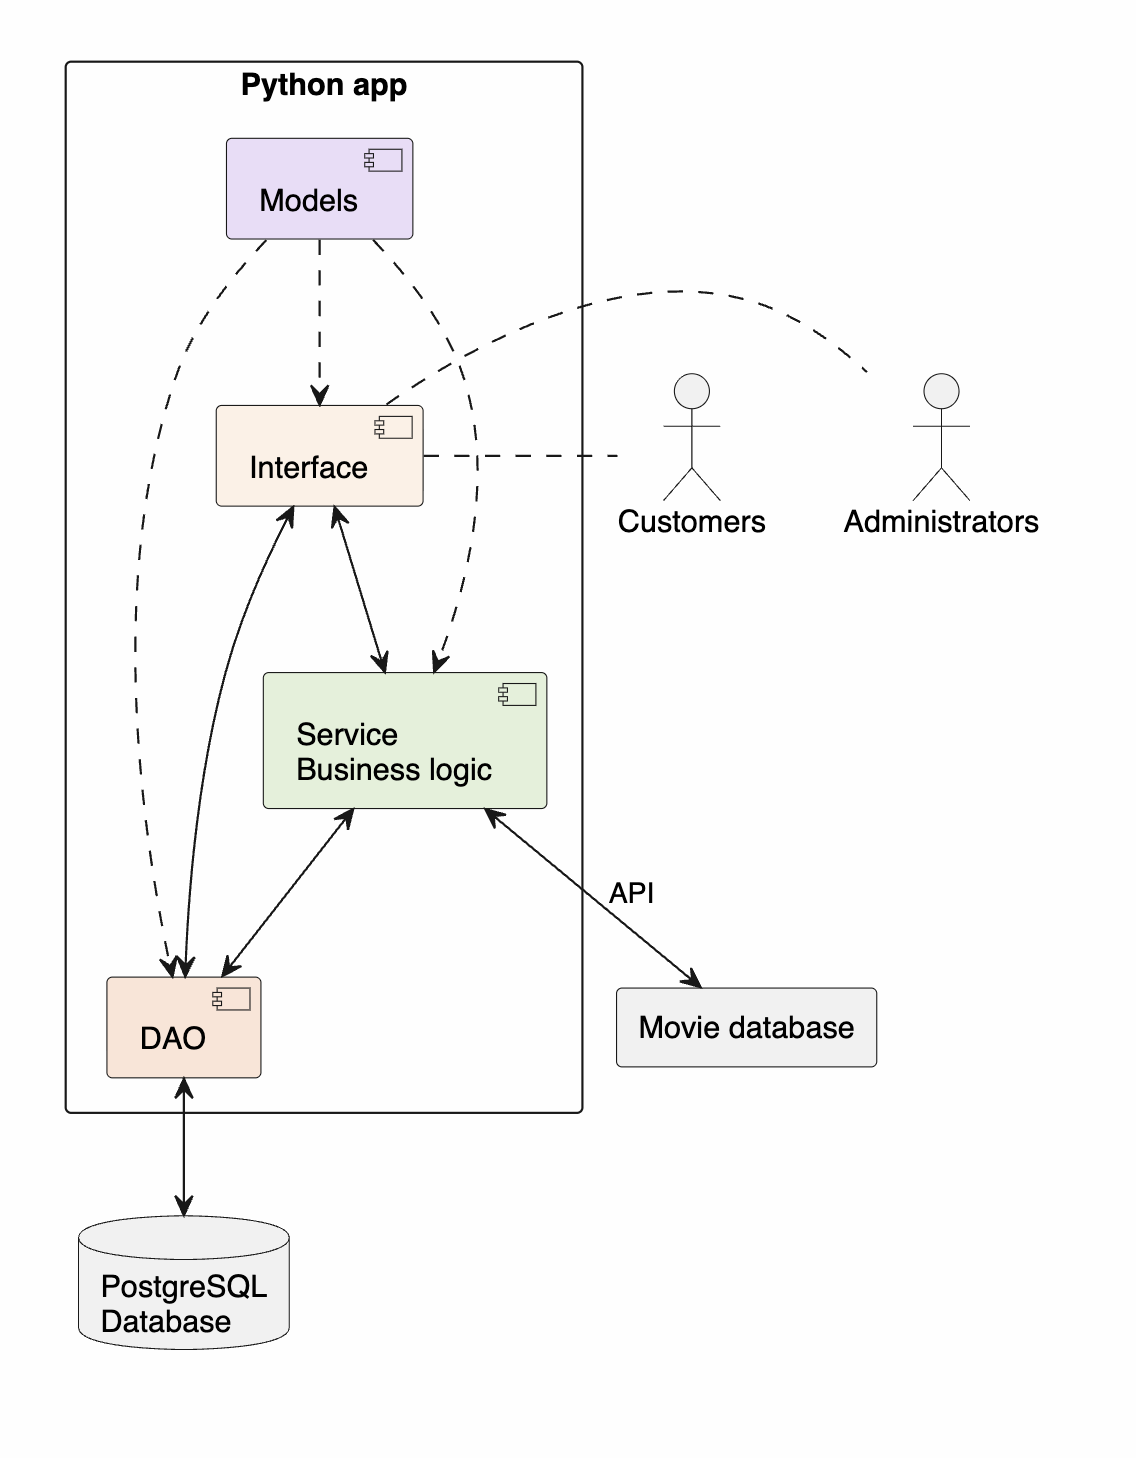
\includegraphics[keepaspectratio]{architecture-diagram.png}}

}

\caption{\label{fig-architecture}Architecture diagram}

\end{figure}%

{[}\emph{Comment on the diagram ( Figure~\ref{fig-architecture}): role
of each layer, technologies used.}{]}

\subsection{Data model}\label{data-model}

\emph{{[}What information does the application need to store? List the
main entities and their attributes.{]}}

: Data model --- main entities

\begin{figure}

\centering{

\pandocbounded{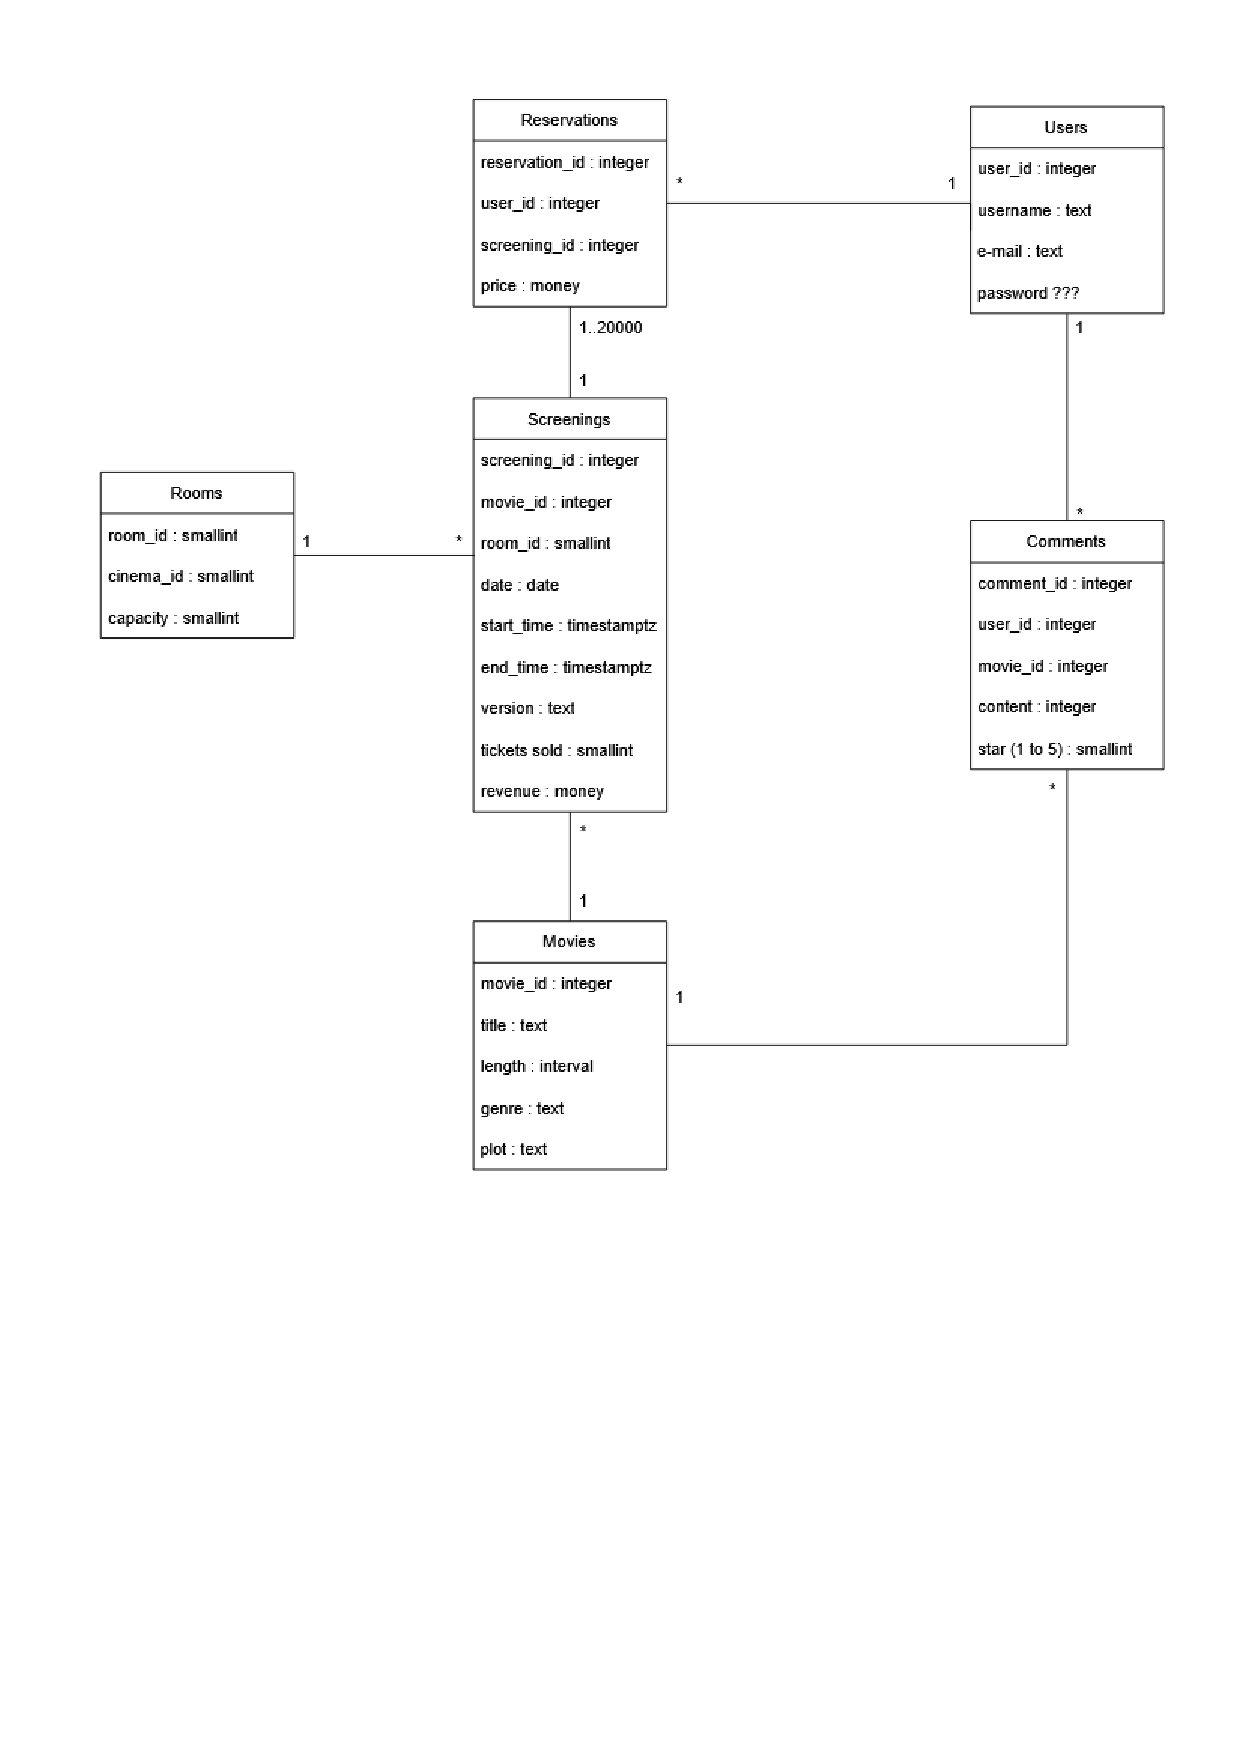
\includegraphics[keepaspectratio]{data model.pdf}}

}

\caption{\label{fig-dm}Data Model}

\end{figure}%

\subsection{Class diagram}\label{class-diagram}

\emph{{[}Object-oriented structure of the application: classes,
attributes, methods, relationships (inheritance, composition,
association).{]}}

{[}\emph{Briefly comment on the main classes and their relationships (
\textbf{?@fig-class}).}{]}

\subsection{Activity diagrams}\label{activity-diagrams}

\begin{figure}

\centering{

\pandocbounded{\includegraphics[keepaspectratio]{.pdf}}

}

\caption{\label{fig-usecase}User activity diagram}

\end{figure}%

\begin{figure}

\centering{

\pandocbounded{\includegraphics[keepaspectratio]{.pdf}}

}

\caption{\label{fig-usecase}Admin activity diagram}

\end{figure}%

\section{Part 4 -- Project Management
Description}\label{part-4-project-management-description}

\subsection{Organization of the team as a product and development
team}\label{organization-of-the-team-as-a-product-and-development-team}

\emph{{[}Presentation of the team: who plays which role on the
``product'' side (vision, prioritization) and on the ``development''
side (implementation).{]}}

\begin{longtable}[]{@{}lll@{}}
\caption{Team organization}\tabularnewline
\toprule\noalign{}
Member & Product role & Development role \\
\midrule\noalign{}
\endfirsthead
\toprule\noalign{}
Member & Product role & Development role \\
\midrule\noalign{}
\endhead
\bottomrule\noalign{}
\endlastfoot
\emph{{[}Name{]}} & \emph{{[}e.g., Product Owner{]}} & \emph{{[}e.g.,
Backend{]}} \\
\emph{{[}Name{]}} & & \\
\end{longtable}

\subsection{Role assignment within the
group}\label{role-assignment-within-the-group}

\emph{{[}Detail of each member's responsibilities, optionally as a RACI
table.{]}}

\begin{longtable}[]{@{}llll@{}}
\caption{Role assignment (RACI)}\tabularnewline
\toprule\noalign{}
Task / Module & Responsible & Contributors & Approved by \\
\midrule\noalign{}
\endfirsthead
\toprule\noalign{}
Task / Module & Responsible & Contributors & Approved by \\
\midrule\noalign{}
\endhead
\bottomrule\noalign{}
\endlastfoot
& & & \\
\end{longtable}

\subsection{Methodology}\label{methodology}

\emph{{[}Working methodology adopted: Agile/Scrum, sprints,
communication tools (Slack, Discord\ldots), task management tools
(Trello, Notion, GitHub Projects\ldots), meeting frequency, code
management (Git workflow, code reviews).{]}}

\subsection{Projected schedule -- Gantt
chart}\label{projected-schedule-gantt-chart}

\emph{{[}Schedule of the project's main milestones up to the November
deadline.{]}}

\begin{figure}

\centering{

\pandocbounded{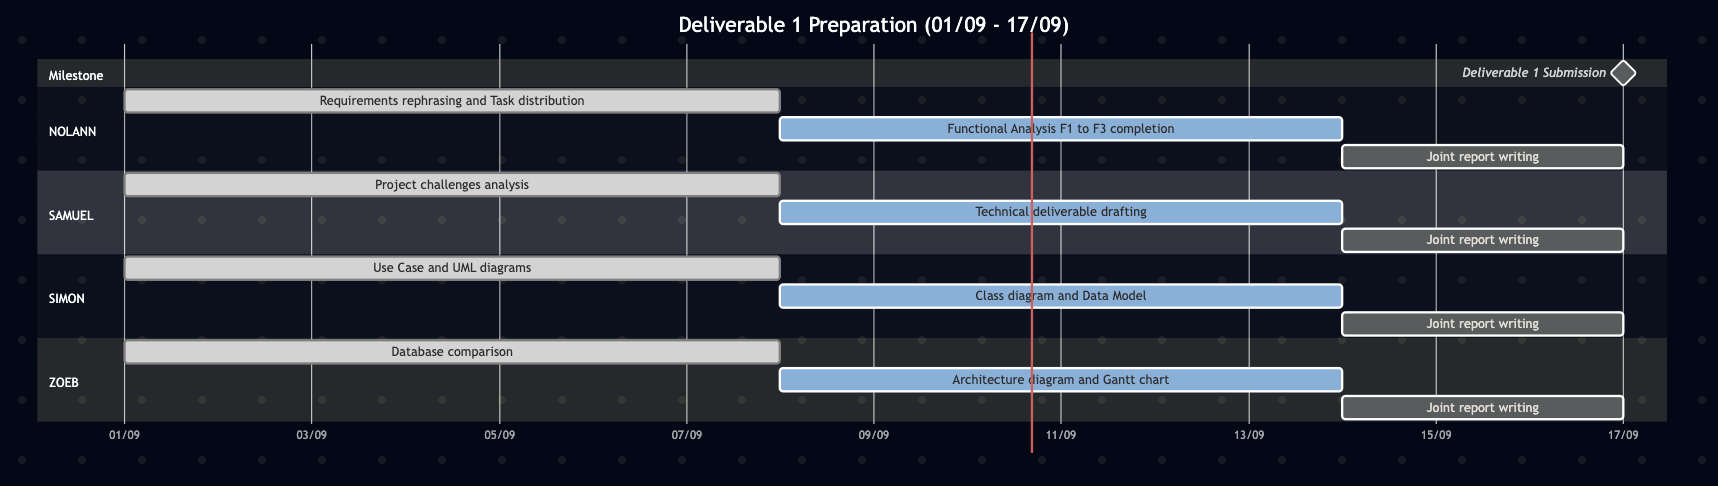
\includegraphics[keepaspectratio]{gantt diagram.png}}

}

\caption{\label{fig-gantt}Gantt chart}

\end{figure}%

\subsection{Challenges encountered and
adjustments}\label{challenges-encountered-and-adjustments}

\emph{{[}Optional: lessons learned on project management, unforeseen
events, schedule or scope adjustments.{]}}

\begin{center}\rule{0.5\linewidth}{0.5pt}\end{center}

\section{Conclusion}\label{conclusion}

\emph{{[}Assessment of the work carried out against the objectives set
in the introduction, review of features actually delivered vs.~planned,
limitations of the project, possible future developments.{]}}

\begin{center}\rule{0.5\linewidth}{0.5pt}\end{center}

\section{Appendices}\label{appendices}

\begin{itemize}
\tightlist
\item
  \emph{{[}Original requirements / brief{]}}
\item
  \emph{{[}Significant code excerpts{]}}
\item
  \emph{{[}Mockups / wireframes{]}}
\end{itemize}




\end{document}
